\section{Control problem}

% Choice of the topic
\subsection{Choice of the topic}
The chosen topic is : {\bf Active mass damper}.

% Context
\subsection{Context}
The current engineering prowesses allow us to construct buildings higher and higher. These constructions are subject to various disturbances (mainly wind, but also earthquakes) that make them oscillate. They turn into giant pendulum and swing from left to right, sometimes moving several meters at the top !\cite{YouTube_minutephysics}\par
To reduce these oscillations, we use a passive system, called {\it tuned mass damper}, which consists of concealing a tuned and harmonic oscillator at the top of the tower. It is coupled to its movement and oscillates in phase opposition to recover the kinetic energy of the tower and thus reduces the oscillations.\cite{Wikipedia_amortisseur_tmd}\par
An active version of this system exists : the {\it active mass damper}. It consists of the same principle as the tuned mass damper but it is equipped with sensors and actuators to measure the oscillations of its environment and, via an algorithm, generate a movement for the mass that reduce, or totally remove, these oscillations.\cite{sciencedirect_amd}\par
Our study field focuses on the active mass damper systems used to reduce the oscillations caused by the {\bf wind} on {\bf tall} buildings.

% Control problem diagram
\subsection{Control problem diagram}
The diagram of our control problem is shown in figure \ref{fig:diagram}.
\begin{figure}[!ht]
    \centering
    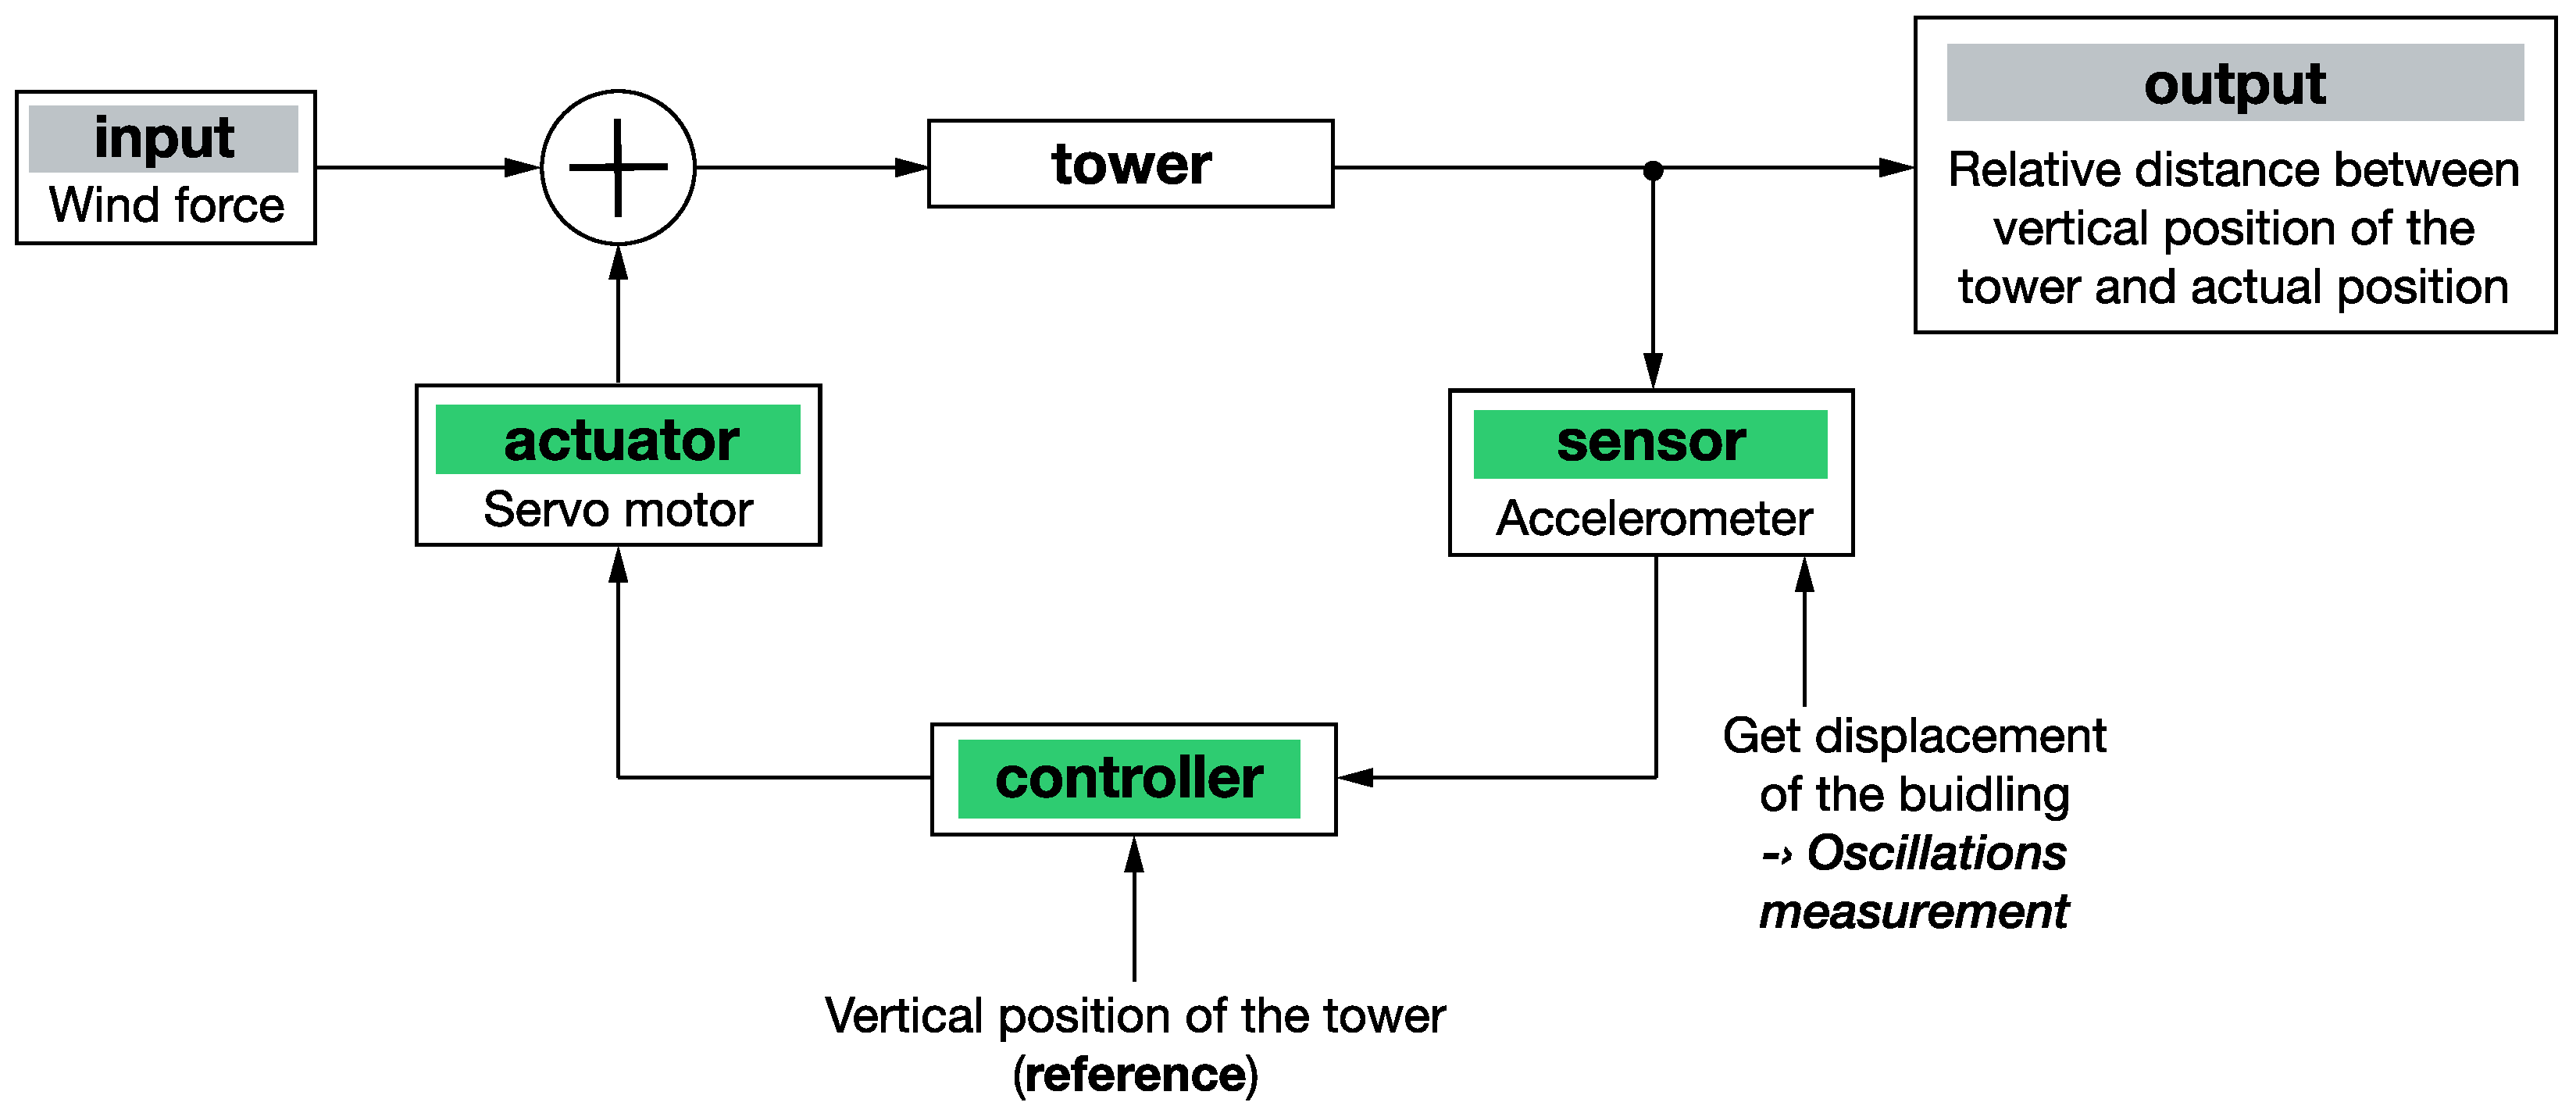
\includegraphics[width=1\textwidth]{resources/pdf/control-problem-diagram.pdf}
    \caption{Control problem diagram of the active mass damper for tall buildings}
    \label{fig:diagram}
\end{figure}

% Control problem description
\subsection{Control problem description}
\begin{itemize}
    \item {\bf Utility of the controller} : the controller (the algorithm) allows the system (the tower) to be active, {\it i.e.} to measure the oscillations to which it is subjected and to cancel it. Thanks to a servo-motor connected to the controller, the mass can move and reduce, or even eliminate totally, the oscillations.
    \item {\bf System to be controlled} : the tower (and the position of the tower is the signal)
    \item {\bf Inputs of the system} : wind force acting on the tower (uncontrollable) and force acting on the mass damper (controllable).
    \item {\bf Outputs of the system} : the relative distance between the vertical position and the displacement of the tower.
    \item {\bf Reference} : the vertical position of the tower.
    \item {\bf Actuators} : servo-motor to move the mass that reduces the oscillations.
    \item {\bf Constraints and limitations} : to simplify our system, we consider a tower \SI{200}{\meter} high, perfectly vertical when it undergoes no disturbance. The only disturbance on this tower is the strength of the wind. The wind, ranging from a few tens of \SI{}{\kilo\meter/\hour} to a hundred \SI{}{\kilo\meter/\hour}, can swing the tower from a few centimetres to several meters.
\end{itemize}

% Open loop system diagram
\subsection{Open loop system diagram}
The detailed schematic of the open loop studied system is shown in figure \ref{fig:detailed_schematic}.
\begin{figure}[H]
    \centering
    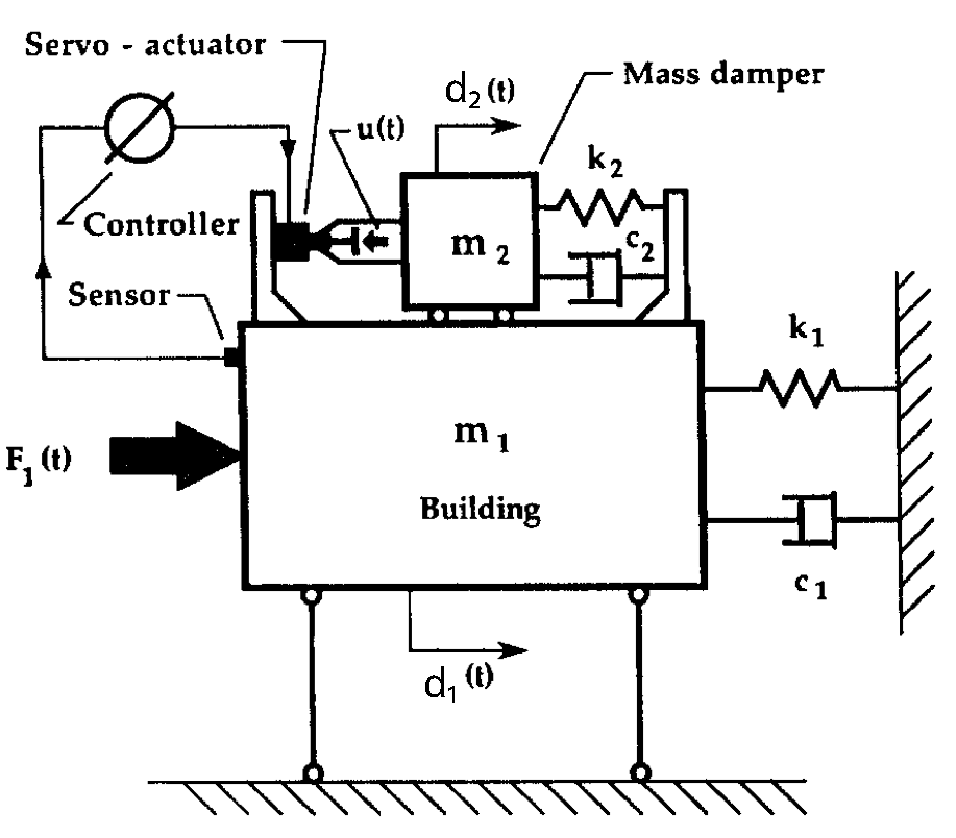
\includegraphics[width=0.7\textwidth]{resources/pdf/open-loop-diagram.pdf}
    \caption{Detailed schematic of the open loop studied system \cite{sciencedirect_amd}}
    \label{fig:detailed_schematic}
\end{figure}
The building is represented by the mass $m_1$ and its oscillation motion is simulated by the spring $k_1$ and the damper $c_1$.\par
The mass damper is represented by the mass $m_2$ and its movement is simulated by the spring $k_2$ and the damper $c_2$.\par
The force $F_1(t)$ represents the wind force (uncontrollable) on the building.\par
The force $u(t)$ represents the force applied on the mass damper by the controller (controllable).\par
We are studying, at first, our system without a control mechanism. Our controllable input $u(t)$ will therefore be \num{0} for all our simulations in this section.
